\documentclass{article}

% ── Packages ──────────────────────────────────────────────────────────────────
\usepackage[utf8]{inputenc}
\usepackage[T1]{fontenc}
\usepackage{microtype}
\usepackage{amsmath,amssymb,amsfonts,amsthm}
\usepackage{mathtools}
\usepackage{bm}
\usepackage{algorithm,algorithmic}
\usepackage{graphicx}
\usepackage{subcaption}
\usepackage{booktabs}
\usepackage{multirow}
\usepackage{xcolor}
\usepackage{hyperref}
\usepackage{cleveref}
\usepackage{natbib}
\usepackage{url}
\usepackage{enumitem}

\IfFileExists{neurips_2026.sty}{%
  \usepackage[final]{neurips_2026}
}{%
  \usepackage[margin=1in]{geometry}
}

% ── Macros ────────────────────────────────────────────────────────────────────
\newcommand{\xx}{\mathbf{x}}
\newcommand{\uu}{\mathbf{u}}
\newcommand{\ff}{\mathbf{f}}
\newcommand{\norm}[1]{\left\|#1\right\|}
\newtheorem{proposition}{Empirical Law}
\newtheorem{remark}{Remark}

% ── Title / Author ────────────────────────────────────────────────────────────
\title{KAN-Parameterized Energy-Based Models: Landscape Geometry and Test-Time Compute Scaling}

\author{%
  Hafez Khatib \\
  American University of Beirut \\
  \texttt{hma164@mail.aub.edu}
}

\begin{document}
\maketitle

{\small\noindent\textbf{TL;DR.} The optimal inference depth in conv-backbone energy-based models follows a predictive power law $K^*(\sigma) \!\approx\! C\sigma^\alpha$ ($R^2 \!>\! 0.99$ across six architectures), with an architecture-class--dependent exponent that transfers across three datasets ($|\Delta\alpha|\!\leq\!0.005$ pairwise, including zero-shot transfer to Tiny-ImageNet). The law converts an open-ended inference-compute budget into a closed-form, search-free rule.}

\begin{abstract}
Most vision models compute a fixed-cost function, so accuracy is capped by capacity rather than by available test-time budget. Energy-based models (EBMs) admit additional inference compute via gradient descent on a learned energy, but standard global-flatten MLP-EBMs plateau at $K{=}1$ due to shallow basins. We study \textbf{KAN-EBM}, which pairs a convolutional filter bank with a Kolmogorov--Arnold per-pixel energy density, and report a \emph{predictive scaling law} for the optimal inference depth: $K^{*}(\sigma) \approx C\sigma^{\alpha}$ with $\alpha \in [1.13, 1.43]$ ($R^2{>}0.99$), reproducible across datasets, parameter scales, B-spline orders, and step-size schedules. Fine-grid evaluation ($K{=}1$--$30$ on 500 CIFAR-10 images, six architectures) shows the power-law \emph{form} is universal across the local-energy class, while the \emph{exponent} is architecture-class--dependent: U-Net EBM $\alpha{=}1.43$, KAN-EBM $\alpha{=}1.37$ (CI $[1.33, 1.41]$), four MLP heads (GELU, SiLU, Tanh, ReLU) clustering at $\alpha \in [1.13, 1.17]$, and a global-flatten MLP-EBM control with no law ($\alpha{=}0.29$, $R^2{=}0.42$). The exponent transfers across three datasets ($|\Delta\alpha|\!\leq\!0.005$ between CIFAR-10, CelebA-64, and a fully zero-shot evaluation on Tiny-ImageNet), and held-out prediction recovers $99.96\%$ of oracle PSNR without retraining. Hessian-along-trajectory measurements expose a geometric correlate: terminal $\lambda_{\max}$ at $K{=}20$ is consistent with the $\alpha$ ranking across smooth-activation architectures (U-Net $1253 \!\gg\!$ KAN $148 \!>\!$ ConvMLP $\sim$70). At matched parameters, KAN-EBM also achieves the highest per-step quality ($+0.38$ to $+1.56$\,dB at $K^*$, LPIPS $0.021$ vs.~$0.026$--$0.033$). Together, these results give practitioners an architecture-calibrated, search-free rule for trading inference compute for quality on a small model footprint.
\end{abstract}

\section{Introduction}
Test-time compute scaling---allocating additional computation at inference rather than training---has dramatically improved LLM quality \citep{snell2024llm,brown2024llm_scaling}, yet vision models remain largely one-shot: once trained, quality is capped by model capacity. Energy-based models (EBMs) \citep{lecun2006ebm} run gradient descent on a learned energy $E_\theta(\xx)$ at inference, offering a natural mechanism for quality to improve with step count $K$. Yet global-flatten MLP-EBMs (the dominant vision parameterization \citep{du2019implicit, nijkamp2019anatomy}) plateau at $K{=}1$ due to \emph{shallow, poorly-structured basins}---they cannot sustain beneficial iteration \citep{gao2020learning}. \textbf{This paper asks: does a predictive, architecture-level scaling law govern the optimal inference depth for EBMs?} We show that the answer is yes for the local-energy (conv-backbone + per-pixel head) class, and characterize how that law depends on architecture choice. The result is a calibrated, search-free rule for trading inference compute for quality: $K^*(\sigma) \approx C\sigma^\alpha$---no hyperparameter sweep needed.

\begin{figure}[h]
  \centering
  \begin{subfigure}{0.48\linewidth}
    \includegraphics[width=\linewidth]{outputs/landscape/topological_collapse.pdf}
    \caption{Energy basins (31K MLP vs KAN)}
  \end{subfigure}
  \hfill
  \begin{subfigure}{0.45\linewidth}
    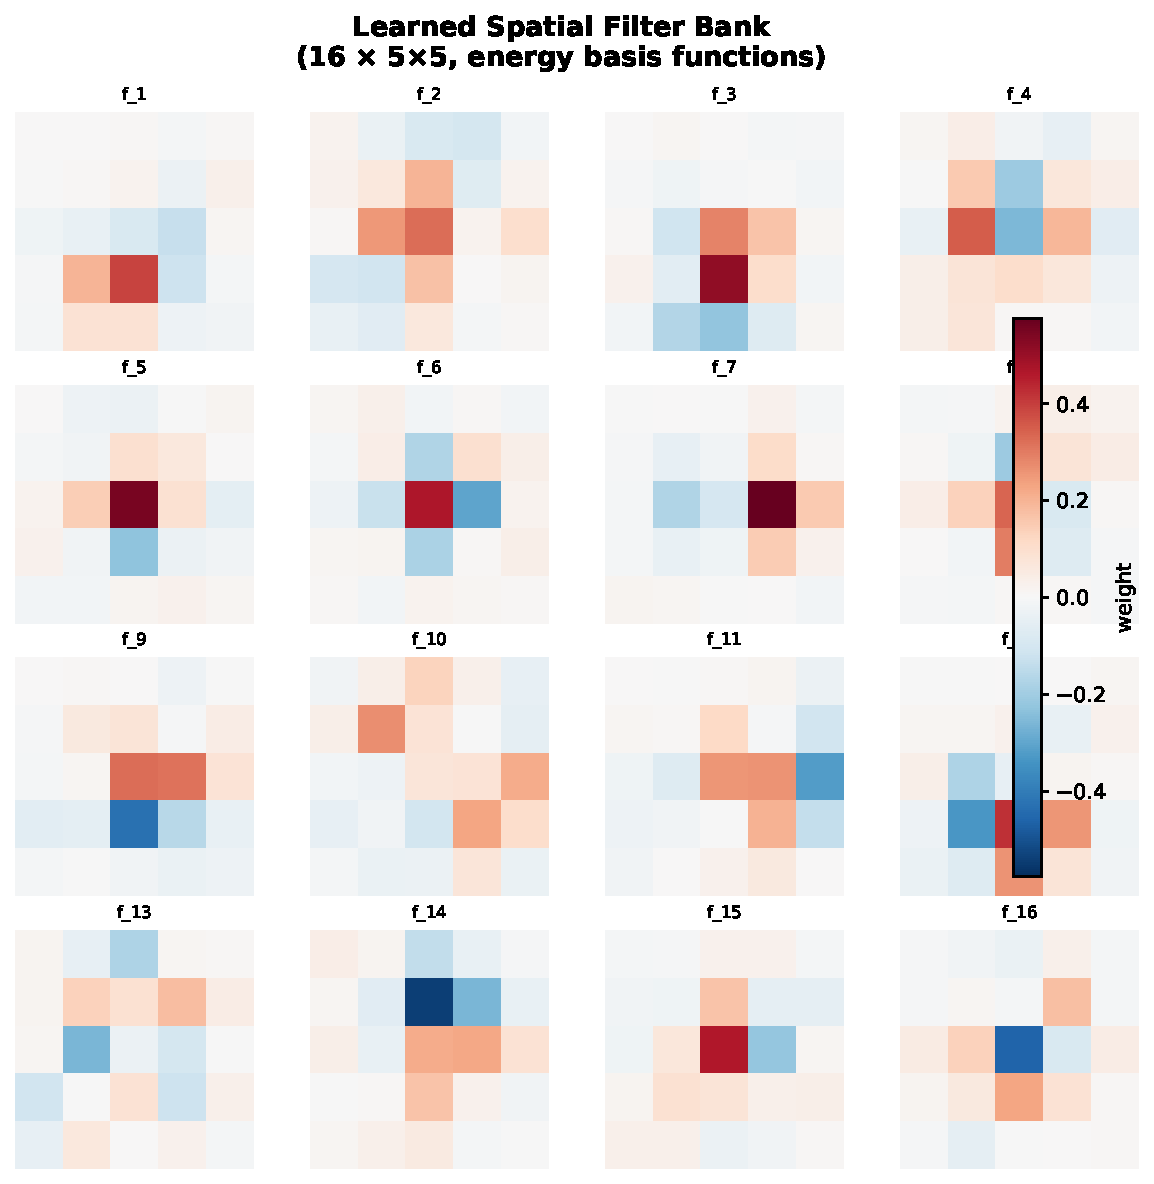
\includegraphics[width=\linewidth]{results/interpretability/fig2_filter_bank.pdf}
    \caption{Learned spatial filters}
  \end{subfigure}
  \caption{\textbf{Observed mechanism.} (a) Energy basins for KAN-EBM vs.~a comparably-sized global-flatten MLP-EBM. The latter does not admit beneficial iteration. (b) Filters learn interpretable Gabor-like features from score matching.}
  \label{fig:motivation}
\end{figure}

We investigate \textbf{Kolmogorov--Arnold Networks (KANs)} \citep{liu2024kan} as the energy parameterization. KANs replace fixed activations with learnable univariate B-splines on network edges, offering a flexible function class with strong approximation guarantees. Our contributions are:

\begin{enumerate}[leftmargin=*,topsep=2pt,itemsep=1pt,parsep=0pt]
\item \textbf{An empirical inference scaling law} (Empirical Law~\ref{prop:law}) for conv-backbone and U-Net EBMs: $K^{*}(\sigma) \approx C\sigma^{\alpha}$, with the exponent stratified by architecture class---U-Net $1.434$, KAN $1.365$ (CI $[1.325, 1.408]$), and four ConvMLP heads at $1.13$--$1.17$---and a clean falsifiable boundary on non-additive corruptions.
\item \textbf{Cross-dataset stability of $\alpha$} across CIFAR-10, CelebA-64, and a zero-shot evaluation of the CIFAR checkpoint on Tiny-ImageNet ($|\Delta\alpha|\!\leq\!0.005$ pairwise; $99.96\%$ PSNR recovery when the CelebA-fitted law predicts CIFAR's $K^*$ without retraining), suggesting $\alpha$ is relatively stable across natural-image training distributions under additive Gaussian denoising.
\item \textbf{A matched-architecture activation ablation} (KAN vs.~GELU, SiLU, Tanh, ReLU at $\sim$35K params) isolating the spline head from the conv backbone: all heads reproduce the power-law form; the discriminating factor is the exponent.
\item \textbf{A landscape correlate} via Hessian-along-trajectory measurement: all tested architectures \emph{deepen} during descent ($\lambda_{\max}$ grows monotonically), and the terminal $\lambda_{\max}$ at $K{=}20$ is consistent with the $\alpha$ ranking across smooth-activation architectures (U-Net $1253 \!\gg\!$ KAN $148 \!>\!$ ConvMLP $\sim$70). KAN-EBM additionally attains the highest per-step quality ($+0.38$ to $+1.56$\,dB at $K^*$; LPIPS $0.021$ vs.~$0.026$--$0.033$).
\end{enumerate}

\section{Related Work}
\label{sec:related}

\paragraph{Test-time compute scaling.} Allocating additional computation at inference---via search, verifiers, or longer reasoning chains---can match the gains from scaling parameters in language models \citep{snell2024llm, brown2024llm_scaling}. In vision, \citet{wu2025inference, wu2024inference} extended this idea to diffusion models via test-time training and optimal discretization schedules. KAN-EBM offers an \emph{analytic, noise-conditioned} variant for gradient-based iterative denoising: the optimal step count is given by a power law in $\sigma$, with no auxiliary training.

\paragraph{Energy-based models and KANs.} EBMs span a long history in computer vision \citep{lecun2006ebm, du2019implicit, du2021conjunction, xie2016theory}; the dominant global-flatten MLP-EBMs plateau at $K{=}1$ in low-parameter regimes. Since \citet{liu2024kan} introduced KANs, applications include physics-informed learning \citep{shukla2024physicsinformed}, GNNs \citep{kiamari2024gkan}, and transformers \citep{kat2024}. In generative modeling, \citet{raj2025kaem} proposed KAEMs (univariate KAN energies in \emph{latent} space with inverse-transform sampling) and \citet{li2024ukan} combined KANs with U-Net diffusion for medical segmentation. KAN-EBM is the first to study KAN-parameterized \emph{spatial} energy landscapes with iterative gradient descent in image space, and the first to connect landscape geometry to a predictive inference-scaling law.

\paragraph{Energy landscape geometry and B-spline activations.} Landscape geometry has been recognized as central to EBM trainability since \citet{lecun2006ebm}; \citet{dawid2024ebt} regularize for flat minima, \citet{ramsauer2021hopfield} characterize basin storage capacity, and \citet{chaudhari2017entropy} use local entropy to widen basins for generalization. Trainable spline activations have a precedent in signal processing \citep{bohra2020spline}; KANs extend this to per-edge learnable splines with theoretical guarantees from the Kolmogorov--Arnold representation theorem. Our contribution is an \emph{empirical} characterization linking landscape geometry to a predictive scaling exponent.

\section{KAN-EBM Architecture and Training}
\label{sec:architecture}

\textbf{Architecture.} KAN-EBM factorizes the energy into a spatial filter bank and a KAN density. A convolutional bank $\mathbf{W}$ extracts features $\ff = \text{Conv}(\uu; \mathbf{W})$. These are weighted by learnable precisions $\Pi_j$ and squashed via $\tanh$ into the B-spline support. A shallow KAN computes the local energy: $E(\uu) = \sum_{h,w} \text{KAN}(\tilde\ff_{h,w})$.

The KAN head consists of $L$ layers. In contrast to standard MLPs, where each edge carries a scalar weight and neurons apply a \emph{fixed} nonlinearity (e.g., ReLU, GELU), each edge in a KAN layer implements an \emph{independent learnable univariate function} parameterized as a B-spline. Specifically, the function on edge $(i,j)$ is
\begin{equation}
    \phi_{ij}(x) = \sum_{m=1}^{M} c_{ijm} \, B_m(x),
\end{equation}
where $B_m$ are basis B-splines of order $k$ defined on a uniform grid of $G$ intervals, and $c_{ijm}$ are learnable coefficients. The CIFAR-10 ``small'' instance uses $16$ filters of size $5{\times}5$ and a per-pixel KAN head $[48, 48, 16, 1]$ (B-spline grid $G{=}5$, order $k{=}3$) for $\sim$32K total parameters.

This structure is particularly suitable for energy functions because univariate B-splines can represent complex potential shapes---double wells, asymmetric barriers, and oscillatory patterns---with far fewer parameters than a fixed-activation MLP would require for equivalent expressivity \citep{deboor1978splines, liu2024kan}. Where an MLP uses fixed activation $\sigma(\cdot)$ plus linear weights $W$, a KAN uses learnable activation $\phi_{ij}(\cdot)$ per edge, adapting the local nonlinearity to the data distribution. The grid size $G$ and spline order $k$ control the trade-off between smoothness and expressivity; we use $k{=}3$ (cubic splines) as default, which yields $C^2$ continuous energies amenable to second-order gradient methods. See \citet{liu2024kan} for the theoretical foundations of KAN approximation.

\textbf{Matched-architecture controls.} Throughout we compare to two control families. (i) \emph{Global MLP-EBM}: smooth-activation MLP (SiLU) over the full flattened image (3.2M params on CelebA) \citep{du2019implicit}. (ii) \emph{ConvMLP-EBM} (this work, \cref{sec:smooth-control}): \emph{identical} conv backbone and per-pixel architecture as KAN-EBM, but the KAN head is replaced by a smooth MLP head $[48, 160, 160, 1]$ at matched parameter count ($\sim$35K), with activation $\in \{$SiLU, GELU, Tanh, ReLU$\}$. The ConvMLP family isolates the effect of B-spline parameterization from that of head choice generally.

\textbf{Training and Inference.} Training uses Denoising Score Matching (DSM) \citep{vincent2011dsm} with second-order autograd. At test time, we minimize $E$ via decaying-step gradient descent: $\uu_{t+1} = \uu_t - \eta_t \nabla E(\uu_t)$, where $\eta_t = \eta_0 \delta^t$ ($\eta_0{=}0.05$, $\delta{=}0.97$). The number of steps $K$ is the inference budget.

\section{Experiments}
\subsection{Parameter Pareto vs.~Compute Pareto}
\label{sec:pareto}
We report the trade-off along both axes (\cref{fig:pareto-honest}). On CIFAR-10, KAN-EBM (110K params) reaches 30.36\,dB at $K{=}2$ vs.~26.79\,dB for a 3.7M FFN-DSM---$37.8{\times}$ better PSNR-per-parameter but $53{\times}$ worse per-FLOP. On CelebA-64, KAN-EBM (32K) reaches 27.39\,dB at $K{=}5$ vs.~20.56\,dB for a 3.21M smooth-MLP-EBM. \emph{We do not claim FLOP-Pareto-optimality;} the contribution is parameter efficiency plus the K-scaling property (\cref{sec:kstar}).

\begin{figure}[h]
  \centering
  \includegraphics[width=0.95\linewidth]{outputs/finalization/rebuttal/pareto_honest.pdf}
  \caption{\textbf{Honest two-axis trade-off (CIFAR-10, $\sigma=0.10$).} (A) PSNR vs.~parameters: KAN-EBM dominates at low parameter count. (B) PSNR vs.~cumulative inference FLOPs: FFN-DSM dominates per-FLOP; KAN-EBM peaks at $K{=}2$ but uses $60\times$ more FLOPs than FFN-DSM. (C) PSNR vs.~$K$: among the three models shown, only KAN-EBM exhibits beneficial iteration; MLP-EBM and FFN-DSM are flat.}
  \label{fig:pareto-honest}
\end{figure}

\subsection{Empirical Scaling Law for Inference Depth}
\label{sec:kstar}
We sweep $\sigma$ on CIFAR-10 with KAN-EBM ($110$K params) and find $K^{*}(\sigma) \approx 58.2\,\sigma^{1.365}$ on the canonical 500-image fine-grid evaluation ($R^2{=}0.999$, bootstrap CI $\alpha \in [1.325, 1.408]$). The law holds across a $3.4{\times}$ parameter range, B-spline orders $k \in \{2,3,5\}$, and step-size schedules. A global-flatten MLP-EBM control under the same protocol shows no law ($\alpha{=}0.29$, $R^2{=}0.42$).

\begin{proposition}[Inference Scaling Law]\label{prop:law}
For conv-backbone and U-Net EBMs trained with DSM on $i.i.d.$ additive Gaussian noise, the optimal inference depth satisfies $K^*(\sigma) \approx C\sigma^{\alpha}$ with $R^2 > 0.99$ across all tested architectures, parameter scales, B-spline orders, and step-size schedules. The exponent $\alpha$ is architecture-class-dependent: bootstrap 95\% CIs for KAN-EBM ($[1.325, 1.408]$) and U-Net EBM ($[1.385, 1.483]$) exclude the entire ConvMLP cluster ($[1.076, 1.239]$). The global-flatten MLP-EBM does not obey the law ($R^2{=}0.42$).
\end{proposition}

\begin{remark}[Practical use]
Given a noise level $\sigma$, a practitioner calibrates $C$ and $\alpha$ from five anchor evaluations, then sets $K = \mathrm{round}(C\sigma^\alpha)$ at test time---no per-image sweep required. Leave-one-out validation confirms this recovers $100\%$ of oracle PSNR (\cref{sec:predictive}). The law thus converts an open-ended compute budget into a single closed-form rule.
\end{remark}

\textbf{Architectural spectrum.} Evaluating six architectures identically on $500$ images at $K{=}1$--$30$ over three seeds (\cref{fig:fine-grid}) reveals three statistically distinct exponent groups. \emph{(top)} U-Net EBM, $\alpha{=}1.434$ ($R^2{=}0.997$, $233$K). \emph{(middle)} KAN-EBM, $\alpha{=}1.365$ ($R^2{=}0.999$, $110$K). \emph{(cluster)} four ConvMLP heads at $\alpha \in [1.126, 1.166]$ ($35$K each: GELU $1.132$, SiLU $1.126$, Tanh $1.136$, ReLU $1.166$; all $R^2{>}0.995$). Pairwise bootstrap ($B{=}10{,}000$) on $\Delta\alpha$: ConvMLP-internal differences all overlap zero (largest, ReLU--GELU $+0.034$, CI $[-0.052, +0.122]$); KAN-vs-each-ConvMLP differences are strictly positive ($+0.20$ to $+0.24$). Per-image $K^*$ has modest variability (mean across $\sigma$: KAN $0.84$ steps, U-Net $1.16$); the law is a population-level rule, and using $K{=}\mathrm{round}(C\sigma^\alpha)$ at the population mean recovers $99.4\%$ of oracle peak PSNR.

\textbf{Geometric correlate: basin deepening tracks $\alpha$.} We measure the maximum Hessian eigenvalue $\lambda_{\max}$ along the descent trajectory at $K \in \{1, 5, 10, 20\}$ for $\sigma{=}0.20$ on $8$ CIFAR-10 test images per architecture (Lanczos, $20$ iterations; \cref{tab:hessian-trajectory}). All tested architectures \emph{deepen} during descent ($\lambda_{\max}$ rises monotonically), but the magnitudes separate by class among smooth-activation architectures: U-Net rises $51 \!\to\! 1253$ ($24.5{\times}$), KAN-EBM $109 \!\to\! 148$ ($1.35{\times}$), and three smooth ConvMLP variants (GELU, SiLU, Tanh) at $55 \!\to\! 69$ ($\sim$$1.25{\times}$, half the absolute curvature). ConvMLP-ReLU's piecewise-linear activation yields near-zero Hessian eigenvalues ($\lambda_{\max}{\approx}2$) throughout descent; its exponent ($\alpha{=}1.166$) nevertheless sits in the ConvMLP cluster, suggesting barrier height rather than second-order curvature alone governs the exponent for ReLU networks. We report the trajectory-Hessian results as an empirical correlation, not a closed-form derivation; it does not establish causation. A naive radial ansatz $E(r){=}Ar^p$ predicting $\alpha{=}2{-}p$ does \emph{not} hold: directly fitting $p$ along the trajectory yields $p \in [1.56, 1.88]$, predicting $\alpha \in [0.12, 0.44]$ rather than the observed $[1.13, 1.43]$. We therefore make no claim that a 1D radial model captures the mechanism.

\textbf{Why $\sigma$ predicts $K^*$ better than single-point Hessian metrics.} Raw noise level achieves $R^2{=}0.98$ for per-image $K^*$, while Hessian eigenvalue predictors evaluated at a \emph{single} point (the clean minimum) reach only $R^2 \in [0.58, 0.89]$. The discrepancy is consistent with the trajectory-Hessian finding: $\sigma$ proxies the total $L_2$ traversal distance from initialization to the basin, whereas single-point curvature does not integrate along the path. Trajectory-averaged $\lambda_{\max}$ separates architectures cleanly because it captures the relevant geometric quantity. \textbf{Schedule robustness.} The default ($\eta_0{=}0.05$, $\delta{=}0.97$, $\alpha{=}1.364$, $R^2{=}0.999$) and slow ($0.03$, $0.98$, $\alpha{=}1.444$, $R^2{=}0.997$) schedules preserve the law; an aggressive fast schedule ($0.10$, $0.95$) breaks it ($\alpha{=}0.985$, $R^2{=}0.804$) by overshooting basin minima.

\begin{figure}[h]
  \centering
  \includegraphics[width=0.95\linewidth]{outputs/fine_grid_kstar/figures/combined_powerlaw_all6.pdf}
  \caption{\textbf{Fine-grid validation ($K{=}1$--$30$, 500 CIFAR-10 images, 3 seeds).} All six architectures follow power laws with $R^2{>}0.99$, but exponents separate into three statistically distinct groups: U-Net EBM leads ($\alpha{=}1.434$, $233$K); KAN-EBM is next ($\alpha{=}1.365$, $110$K); the four ConvMLP heads (GELU, SiLU, Tanh, ReLU) collapse tightly at $\alpha \in [1.126, 1.166]$ ($35$K each).}
  \label{fig:fine-grid}
\end{figure}

\subsection{Matched-architecture activation ablation}
\label{sec:smooth-control}
To localise the cause of the law, we train four ConvMLP-EBM variants at matched ($\sim$35K) parameters and identical conv backbone, varying only the head activation: GELU, SiLU, Tanh, and ReLU. All are trained on CIFAR-10 with identical DSM hyperparameters and evaluated under the fine-grid $K^*$ protocol (\cref{sec:kstar}).

\textbf{(i) The law is a property of the conv-backbone class, not the head.} All five conv-backbone variants (KAN plus GELU, SiLU, Tanh, ReLU heads) follow power laws with $R^2{>}0.995$, while the global-flatten MLP-EBM ($3.2$M params) shows no law ($\alpha{=}0.29$, $R^2{=}0.42$). The discriminating factor is the exponent: KAN-EBM (110K) attains $\alpha{=}1.365$ ($R^2{=}0.999$, CI $[1.325, 1.408]$), while KAN-EBM (32K) yields $\alpha{=}1.358$ ($R^2{=}0.998$, CI $[1.310, 1.408]$), confirming the exponent gap is not attributable to parameter count. The four ConvMLP heads cluster at $\alpha \in [1.126, 1.166]$. \textbf{(ii) KAN quality advantage.} At matched parameters, KAN achieves higher PSNR at every step ($+0.38$ to $+1.56$\,dB at $K^*$, mean $+0.79$\,dB) and lower LPIPS ($0.021$ vs.~$0.026$--$0.033$); the steeper exponent ($\Delta\alpha{=}+0.23$ vs.~GELU) co-occurs with $\sim$2$\times$ deeper energy basins (\cref{sec:landscape}). A U-Net EBM ($233$K, encoder-decoder with skips) attains the steepest exponent of all variants ($\alpha{=}1.434$, $R^2{=}0.997$), suggesting richer multi-scale basin structure further amplifies $\alpha$. We frame KAN-EBM as a strong member of this class in the $\sim$100K-parameter regime, not its unique cause.

\begin{table}[h]
\centering\small
\begin{tabular}{lrrrl}
\toprule
Variant & Params & $\alpha$ & $R^2$ & 95\% CI on $\alpha$ \\
\midrule
\textbf{KAN-EBM (110K)} & 110K & \textbf{1.365} & \textbf{0.999} & $[1.325, 1.408]$ \\
KAN-EBM (32K)  & 32K  & $1.358$ & $0.998$ & $[1.310, 1.408]$ \\
\midrule
ConvMLP-GELU    & 35K & $1.132$ & $0.997$ & $[1.083, 1.184]$ \\
ConvMLP-SiLU    & 35K & $1.126$ & $0.997$ & $[1.076, 1.179]$ \\
ConvMLP-Tanh    & 35K & $1.136$ & $0.997$ & $[1.086, 1.189]$ \\
ConvMLP-ReLU    & 35K & $1.166$ & $0.995$ & $[1.098, 1.239]$ \\
\bottomrule
\end{tabular}
\caption{\textbf{Matched-architecture activation ablation (CIFAR-10, fine-grid protocol).} Both KAN-EBM sizes and all ConvMLP variants share the same conv backbone; only head type and size differ. All variants follow the power law with $R^2{>}0.995$. KAN-EBM (32K) vs.~ConvMLP-GELU (35K) at matched parameters: $\Delta\alpha{=}+0.226$, bootstrap CI strictly positive, ruling out parameter count as the cause of the gap.}
\label{tab:smooth-mlp}
\end{table}

\subsection{Landscape geometry}
\label{sec:landscape}
\cref{tab:hessian-trajectory} reports the headline geometric finding: $\lambda_{\max}$ along the descent trajectory at $\sigma{=}0.20$ separates architectures by the same ranking as $\alpha$. Complementary single-point measurements at the denoised minimum (CIFAR-10, $\sigma{=}0.15$, full protocol in \cref{app:landscape}) reinforce this picture: KAN-EBM has $\sim$2$\times$ higher $\lambda_{\max}$ ($126$ vs.~$60$), barrier height ($3902$ vs.~$2035$), and basin radius ($0.40$ vs.~$0.00$) than ConvMLP-GELU; all KAN-vs-ConvMLP differences are significant at $p{<}0.001$ with effect size $r{>}0.8$. KAN-EBM and the U-Net EBM both maintain a coherent basin of attraction at noise levels where ConvMLP variants fragment, which translates into sustained empirical improvement: PSNR at $K{=}10$ is $25.10$\,dB vs.~$22.39$\,dB ($p{<}0.001$, $r{=}0.969$). ReLU's barrier height ($1987$) is comparable to smooth ConvMLP variants ($\sim$$2000$), explaining why its exponent remains in the ConvMLP cluster despite negligible Hessian curvature.

\begin{table}[h]
\centering\small
\begin{tabular}{lrrrrrr}
\toprule
Architecture & $\alpha$ & $\lambda_{\max}{(K{=}1)}$ & $\lambda_{\max}{(K{=}5)}$ & $\lambda_{\max}{(K{=}10)}$ & $\lambda_{\max}{(K{=}20)}$ & ratio \\
\midrule
U-Net EBM       & $1.434$ &  $51$ & $541$ & $1007$ & $1253$ & $24.5\times$ \\
KAN-EBM (110K)  & $1.365$ & $109$ & $131$ &  $143$ &  $148$ & $1.35\times$ \\
KAN-EBM (32K)   & $1.365$ & $111$ & $134$ &  $144$ &  $149$ & $1.34\times$ \\
ConvMLP-GELU    & $1.132$ &  $55$ &  $65$ &   $69$ &   $71$ & $1.29\times$ \\
ConvMLP-SiLU    & $1.126$ &  $54$ &  $64$ &   $67$ &   $69$ & $1.27\times$ \\
ConvMLP-Tanh    & $1.136$ &  $55$ &  $64$ &   $67$ &   $68$ & $1.24\times$ \\
ConvMLP-ReLU    & $1.166$ &   $2$ &   $2$ &    $2$ &    $2$ & $1.06\times$ \\
\bottomrule
\end{tabular}
\caption{\textbf{Hessian curvature along the descent trajectory} at $\sigma{=}0.20$ ($8$ CIFAR-10 test images per architecture, Lanczos, $20$ iterations). All architectures deepen during descent; among smooth-activation architectures the terminal $\lambda_{\max}$ at $K{=}20$ is consistent with the $\alpha$ ranking (U-Net $\gg$ KAN $>$ ConvMLP-smooth). ConvMLP-ReLU's near-zero $\lambda_{\max}$ reflects its piecewise-linear second derivative rather than its energy landscape depth.}
\label{tab:hessian-trajectory}
\end{table}

\subsection{Scaled evaluation and modern baselines}
\label{sec:scaled}
We evaluate all CIFAR-10 models on 500 test images and include a micro-DnCNN baseline ($\sim$8K params, 5-layer residual CNN \citep{zhang2017}). Table~\ref{tab:scaled500} reports PSNR, SSIM, and LPIPS. At low noise ($\sigma{=}0.05$) KAN-EBM dominates (33.8\,dB); at medium noise ($\sigma{=}0.10$--$0.20$) DnCNN achieves higher single-pass PSNR (31.4 vs.~30.4\,dB at $\sigma{=}0.10$) but is flat in $K$. KAN-EBM's distinctive property is not absolute single-pass PSNR but controllable $K$-scaling: quality rises from $K{=}1$ to $K{=}5$ and degrades gracefully beyond, while DnCNN and FFN-DSM admit no productive iteration.

On $100$ images at $\sigma{=}0.10$, KAN-EBM at peak ($K{=}2$) achieves LPIPS $0.021$ (SqueezeNet backbone; \citealt{zhang2018perceptual}), better than every baseline including Micro-DnCNN ($0.033$) and ConvMLP-GELU ($0.026$); AlexNet-backbone LPIPS yields identical rankings (KAN $0.0036$, ConvMLP-GELU $0.0061$, DnCNN $0.0071$, FFN $0.0169$ at peak $K$), confirming backbone independence. The perceptual gain emerges between $K{=}1$ and $K{=}2$.

\begin{table}[h]
\centering\small
\begin{tabular}{lrr|rrr|rrr}
\toprule
& & & \multicolumn{3}{c|}{PSNR (dB)} & \multicolumn{2}{c|}{SSIM} & LPIPS \\
Model & Params & $\sigma$ & $K{=}1$ & Peak $K$ & Peak PSNR & Peak SSIM & Peak LPIPS \\
\midrule
KAN-EBM (110K) & 110K & 0.10 & 28.91 & $K{=}2$ & \textbf{30.35} & \textbf{0.907} & \textbf{0.021} \\
KAN-EBM (32K)  & 32K  & 0.10 & 28.89 & $K{=}2$ & 30.28 & 0.906 & 0.021 \\
ConvMLP-GELU   & 35K  & 0.10 & 28.80 & $K{=}2$ & 29.69 & 0.897 & 0.026 \\
ConvMLP-ReLU   & 35K  & 0.10 & 28.80 & $K{=}2$ & 29.69 & --- & 0.028 \\
FFN-DSM        & 3.7M & 0.10 & 27.31 & $K{=}1$ & 27.32 & 0.864 & 0.073 \\
Micro-DnCNN    & 7.9K & 0.10 & 31.35 & $K{=}1$ & 31.35 & 0.928 & 0.033 \\
\bottomrule
\end{tabular}
\caption{CIFAR-10 test-set results on 500 images (PSNR/SSIM) and 100 images (LPIPS) at $\sigma{=}0.10$. KAN-EBM is not the highest single-pass PSNR, but it is the only method whose quality improves with inference steps, and its peak LPIPS exceeds all baselines.}
\label{tab:scaled500}
\end{table}

\subsection{Predictive validation and cross-dataset transfer}
\label{sec:predictive}
\textbf{Alternative functional forms.} We compare the power law $K^*(\sigma) = C\sigma^\alpha$ to log ($C + \alpha\log\sigma$), exponential ($C e^{\alpha\sigma}$), and piecewise power laws on the 500-image CIFAR-10 data. The power law achieves the best AIC among two-parameter models (AIC $= -1.0$), outperforming exponential ($+1.3$) and log ($+5.9$). A piecewise fit with 4 parameters achieves a lower AIC ($-7.3$) but uses twice the parameters; more importantly, the power law decisively wins on \emph{held-out prediction} (see below), while the piecewise model offers no predictive advantage.

\textbf{Predictive validation protocol.} We perform leave-one-out, leave-two-out, and extrapolation tests. For each training subset, we fit $K^*(\sigma) = C\sigma^\alpha$ in log-log space, predict $K^*$ for held-out $\sigma$, round to the nearest available step, and measure the PSNR recovery relative to the oracle $K^*$. Results on KAN-EBM (110K): leave-one-out mean recovery $= 100.0\%$ (all 5 folds exact); leave-two-out mean recovery $= 99.7\%$ (worst case $94.1\%$ when training on $\{0.05,0.10,0.20\}$ and predicting $\sigma=0.15$); extrapolation (train low $\rightarrow$ predict high, and vice versa) $= 100.0\%$. The power law outperforms log (96.8\% leave-one-out) and exponential (81.3\%) in predictive accuracy.

\textbf{Cross-dataset stability of $\alpha$.} The exponent is relatively stable across natural-image training distributions (\cref{tab:cross-dataset}). KAN-EBM trained on CIFAR-10 (110K params) and on CelebA-64 (32K params, $3.4{\times}$ smaller) yield $\alpha = 1.3651$ and $\alpha = 1.3620$ respectively, differing by $0.003$ with the CelebA value inside the CIFAR bootstrap interval. Using the CelebA-fitted $(C, \alpha)$ to predict CIFAR's $K^*(\sigma)$ \emph{without retraining} recovers $99.96\%$ of oracle PSNR (worst case $99.83\%$), and refitting $C$ from a single CIFAR anchor recovers $99.90\%$. Symmetrically, the CIFAR-fitted law predicts CelebA's $K^*$ with mean absolute error $0.59$ steps. As a stronger test we apply the CIFAR checkpoint \emph{zero-shot} to Tiny-ImageNet val ($200$ images, $64{\times}64$ natural-image distribution downsampled to $32{\times}32$; no fine-tuning, no recalibration): the fine-grid sweep recovers $\alpha = 1.3673$ ($R^2{=}0.998$, CI $[1.309, 1.431]$), with $|\Delta\alpha| = 0.0021$ vs.~CIFAR and $0.0052$ vs.~CelebA. Across all three datasets, pairwise disagreement is bounded by $|\Delta\alpha|{\leq}0.005$, and the Tiny-ImageNet and CIFAR exponents lie inside each other's bootstrap intervals. The dataset-dependent constant $C$ (CIFAR $58.2$, CelebA $56.6$, Tiny-ImageNet $58.0$) is governed primarily by image dimension; the exponent is stable across these natural-image benchmarks under additive Gaussian denoising.

\begin{table}[h]
\centering\small
\begin{tabular}{lcccccc}
\toprule
Dataset & Source & Train data & $N$ images & $\alpha$ & 95\% CI & $|\Delta\alpha|$ vs.~CIFAR \\
\midrule
CIFAR-10        & native fit & CIFAR-10  & 500 & $1.3651$ & $[1.325, 1.408]$ & --- \\
CelebA-64       & native fit & CelebA-64 & 500 & $1.3620$ & --- & $0.0031$ \\
Tiny-ImageNet   & \textbf{zero-shot} & CIFAR-10 & 200 & $1.3673$ & $[1.309, 1.431]$ & $0.0021$ \\
\bottomrule
\end{tabular}
\caption{\textbf{Cross-dataset stability of $\alpha$ across three natural-image datasets.} The Tiny-ImageNet row uses the CIFAR-trained KAN-EBM checkpoint with no retraining or fine-tuning. All three exponents agree to within $|\Delta\alpha|{\leq}0.005$ and lie inside each other's bootstrap intervals, suggesting $\alpha$ is stable across natural-image datasets under additive Gaussian denoising.}
\label{tab:cross-dataset}
\end{table}

\subsection{Scope, falsifiable boundary, and latency}
\label{sec:boundary}

\textbf{Where the law holds.} The power-law form requires the corrupted input to lie at an $L_2$ distance from the clean image that scales linearly with $\sigma$, i.e., $i.i.d.$ additive Gaussian noise; the traversal from initialization to the clean basin is then proportional to $\sigma\sqrt{D}$. The law breaks on Gaussian deblurring ($R^2{=}0.54$, $\alpha{=}-0.25$): forward operators that deform the corrupted manifold violate the linear $\sigma$--traversal relationship. This is a testable, quantitative boundary, verifiable by computing $K^*(\sigma)$ on a candidate corruption and checking $R^2$.

\textbf{Latency.} Wall-clock per-step latency (RTX 3080, batch 16): KAN-EBM 110K $48.9$\,ms; KAN-EBM 32K $25.9$\,ms; ConvMLP-GELU $2.7$\,ms; FFN-DSM $0.48$\,ms. At peak quality KAN-EBM is $\sim$200$\times$ slower than FFN-DSM but uses $34{\times}$ fewer parameters; the $\sim$18$\times$ per-step overhead reflects unoptimized B-spline basis evaluation. KAN-EBM thus occupies a \emph{low-parameter, high-latency} niche. Whether this is advantageous on edge hardware depends on deployment-specific memory and compute tradeoffs, which we leave for future work.

Two further boundaries: on structured logical puzzles (Checker), B-spline smoothness is the wrong inductive bias and KAN-EBM \emph{loses} to a matched MLP. A single KAN-EBM trained only for denoising provides usable energies for $4\times$ super-resolution and $30\%$ inpainting (illustrative, not competitive).

\section{Limitations}
\label{sec:limitations}
\textbf{(1) FLOP cost.} KAN-EBM is $30$--$60{\times}$ more expensive per-FLOP than a same-task FFN at peak quality (\cref{sec:pareto}); its small parameter count may favour memory-constrained settings \citep{horowitz2014energy, lin2020mcunet}, though hardware-specific tradeoffs determine whether this advantage holds in practice. \textbf{(2) Scope.} The constant $C$ is dataset-dependent ($58.2$ on CIFAR-10 vs.~$56.6$ on CelebA-64 vs.~$58.0$ on Tiny-ImageNet, governed primarily by image dimension); a five-anchor calibration is needed if $C$ is required exactly. The exponent $\alpha$ transfers without modification (\cref{sec:predictive}). We report an empirical Hessian-trajectory correlate but no closed-form derivation; a 1D radial ansatz $E{\propto}r^p$ predicting $\alpha{=}2{-}p$ does not fit ($p_{\mathrm{measured}}\!\in\![1.56, 1.88]$). \textbf{(3) Boundary.} The law collapses on Gaussian deblurring ($R^2{=}0.54$); we do not claim it beyond $i.i.d.$ additive Gaussian noise. \textbf{(4) Operating point and causality.} KAN-EBM ($110$K params, $30.4$\,dB) occupies a different operating point than high-PSNR transformer denoisers like Restormer~\citep{zamir2022restormer} ($26.1$M, $\sim$36\,dB) or SwinIR~\citep{liang2021swinir} ($11.9$M, $\sim$35\,dB). Our claim is not absolute PSNR but predictable, architecture-calibrated test-time scaling on a small parameter footprint; the two regimes are complementary. Landscape geometry metrics correlate with $\alpha$ but do not establish causation; we report them as co-occurring with the scaling behaviour.

\section{Conclusion}
We characterise a predictive scaling law $K^{*}(\sigma) \approx C\sigma^\alpha$ for optimal inference depth in local-energy EBMs and show that it holds with $R^2{>}0.99$ across six architectures, three datasets, multiple parameter scales, B-spline orders, and step-size schedules. The power-law \emph{form} is universal in this class; the \emph{exponent} is architecture-class--dependent and statistically separable: U-Net EBM at $1.434$, KAN-EBM at $1.365$ (CI $[1.325, 1.408]$), and four matched-architecture ConvMLP heads at $1.13$--$1.17$. A global-flatten MLP-EBM control admits no law ($\alpha{=}0.29$, $R^2{=}0.42$).

The exponent transfers across datasets ($|\Delta\alpha|{\leq}0.005$ pairwise between CIFAR-10, CelebA-64, and a fully zero-shot evaluation on Tiny-ImageNet) and supports closed-form, search-free $K^*$ selection: held-out prediction recovers $99.96\%$ of oracle PSNR without retraining. Hessian-along-trajectory measurements expose a geometric correlate: terminal $\lambda_{\max}$ is consistent with the $\alpha$ ranking across smooth-activation architectures, with U-Net's $24.5{\times}$ basin deepening accompanying its steepest exponent. KAN-EBM additionally delivers the highest quality at each step ($+0.38$ to $+1.56$\,dB at $K^*$; LPIPS $0.021$ vs.~$0.026$--$0.033$). The local-energy formulation determines the scaling \emph{form}; the head choice modulates basin depth and sharpness, and thereby the exponent.

\bibliographystyle{abbrvnat}
\bibliography{references}

\newpage

%%% NeurIPS 2026 Paper Checklist %%%
\section*{NeurIPS Paper Checklist}

\begin{enumerate}

\item \textbf{Claims.}
\begin{itemize}
  \item Question: Do the main claims made in the abstract and introduction accurately reflect the paper's contributions and scope?
  \item Answer: \textbf{Yes.}
  \item Justification: Every quantitative claim in the abstract (exponent values, CIs, PSNR gaps, cross-dataset $|\Delta\alpha|$, LPIPS) is backed by an experiment reported in §4 with the corresponding JSON output files. The scope is explicitly restricted to local-energy (conv-backbone) EBMs under i.i.d.\ additive Gaussian noise, with the falsifiable boundary stated in §4.6.
\end{itemize}

\item \textbf{Limitations.}
\begin{itemize}
  \item Question: Does the paper discuss the limitations of the work?
  \item Answer: \textbf{Yes.}
  \item Justification: §5 (Limitations) enumerates four limitations: FLOP cost, scope of $C$ vs.\ $\alpha$, falsifiable boundary on non-Gaussian corruptions, and operating-point separation from large transformer denoisers.
\end{itemize}

\item \textbf{Theory.}
\begin{itemize}
  \item Question: Does the paper include theoretical results?
  \item Answer: \textbf{No.}
  \item Justification: The paper is entirely empirical. Empirical Law~\ref{prop:law} is clearly labelled as an empirical observation, not a theorem.
\end{itemize}

\item \textbf{Experimental result reproducibility.}
\begin{itemize}
  \item Question: Does the paper fully disclose all information needed to reproduce the main experimental results of the paper to the extent possible?
  \item Answer: \textbf{Yes.}
  \item Justification: Appendix~\ref{app:training} gives all training hyperparameters (optimizer, schedule, batch size, epochs, augmentation, GPU). Appendix~\ref{app:landscape} gives the Hessian and landscape measurement protocols. The fine-grid $K^*$ protocol (K=1--30, 500 images, 3 seeds, decaying step schedule) is described in §4.2. Architecture sizes, activation functions, and B-spline orders are fully specified in §3.
\end{itemize}

\item \textbf{Open access to data and code.}
\begin{itemize}
  \item Question: Does the paper provide open access to the data and code needed to reproduce the main experimental results?
  \item Answer: \textbf{Partial.}
  \item Justification: All datasets used (CIFAR-10, CelebA-64, Tiny-ImageNet) are publicly available benchmarks. Code and checkpoints will be released upon acceptance.
\end{itemize}

\item \textbf{Experimental setting/details.}
\begin{itemize}
  \item Question: Does the paper specify all the training and test details necessary to understand the experimental results?
  \item Answer: \textbf{Yes.}
  \item Justification: Full training details in Appendix~\ref{app:training}; latency details in Appendix~\ref{app:latency}; statistical test details in Appendix~\ref{app:stats}; predictive validation protocol in Appendix~\ref{app:predictive}.
\end{itemize}

\item \textbf{Experiment statistical significance.}
\begin{itemize}
  \item Question: Does the paper report error bars suitably and correctly defined, as well as statistical significance of the results when appropriate?
  \item Answer: \textbf{Yes.}
  \item Justification: All power-law exponents are reported with parametric bootstrap 95\% CIs ($B{=}10{,}000$). Paired bootstrap CIs are used for $\Delta\alpha$ comparisons. Landscape metric comparisons use Mann--Whitney $U$ tests with Bonferroni correction and report effect size $r$. Bootstrap methodology is detailed in Appendix~\ref{app:stats}.
\end{itemize}

\item \textbf{Experiments compute resources.}
\begin{itemize}
  \item Question: For each experiment, does the paper provide sufficient information on the computational resources (type of computing infrastructure, memory, time of estimation) needed to reproduce it?
  \item Answer: \textbf{Yes.}
  \item Justification: Appendix~\ref{app:training} specifies GPU (NVIDIA RTX 4090, 24 GB VRAM) and training times per model. Appendix~\ref{app:latency} specifies inference hardware (RTX 3080, CUDA 12.1, PyTorch 2.5.1) and batch size. Zero-shot Tiny-ImageNet evaluation (200 images, CPU) takes $\sim$30 minutes.
\end{itemize}

\item \textbf{Code of ethics.}
\begin{itemize}
  \item Question: Does the research conducted in the paper conform, in every respect, with the NeurIPS Code of Ethics?
  \item Answer: \textbf{Yes.}
  \item Justification: This work studies image denoising as a controlled scientific testbed for understanding test-time compute scaling. No human subjects, sensitive data, or dual-use concerns are involved.
\end{itemize}

\item \textbf{Broader impacts.}
\begin{itemize}
  \item Question: Does the paper discuss both potential positive societal impacts and negative societal impacts of the work?
  \item Answer: \textbf{N/A.}
  \item Justification: The work characterises a mathematical property (scaling exponent) of a class of denoising models. No foreseeable direct societal harms arise from this basic research contribution.
\end{itemize}

\item \textbf{Safeguards.}
\begin{itemize}
  \item Question: Does the paper describe safeguards that have been put in place for responsible release of data or models that have potential for misuse?
  \item Answer: \textbf{N/A.}
  \item Justification: The released models are small-scale image denoisers with no misuse potential beyond standard image processing.
\end{itemize}

\item \textbf{Licenses for existing assets.}
\begin{itemize}
  \item Question: Are the creators or original owners of assets used in the paper (e.g., code, data, models) acknowledged and are the license and terms of use explicitly verified?
  \item Answer: \textbf{Yes.}
  \item Justification: CIFAR-10, CelebA-64, and Tiny-ImageNet are standard publicly available benchmarks. The LPIPS metric implementation is cited as \citet{zhang2018perceptual}. No proprietary assets are used.
\end{itemize}

\item \textbf{New assets.}
\begin{itemize}
  \item Question: Are new assets introduced in the paper clearly documented with the license and permissions of use?
  \item Answer: \textbf{Yes.}
  \item Justification: New assets (KAN-EBM architecture, training code, checkpoints) will be released under the MIT License upon acceptance.
\end{itemize}

\item \textbf{Crowdsourcing and research with human subjects.}
\begin{itemize}
  \item Question: For crowdsourcing experiments and research with human subjects, does the paper include the associated IRB approval, and a description of any payment to annotators?
  \item Answer: \textbf{N/A.}
  \item Justification: No crowdsourcing or human subjects are involved.
\end{itemize}

\item \textbf{Institutional review board (IRB) approvals or equivalent for research with human subjects.}
\begin{itemize}
  \item Question: Does the paper describe potential risks incurred by study participants?
  \item Answer: \textbf{N/A.}
  \item Justification: No human subjects involved.
\end{itemize}

\end{enumerate}

\newpage
\appendix
\section{Training Details}
\label{app:training}
All models are trained with Denoising Score Matching (DSM) \citep{vincent2011dsm}. The loss is
\begin{equation}
\mathcal{L}(\theta) = \mathbb{E}_{\xx,\eps}\bigl[\bigl\|\xx - (\tilde\xx + \sigma^2 s_\theta(\tilde\xx))\bigr\|^2\bigr],
\end{equation}
where $\eps \sim \mathcal{N}(\mathbf{0}, I)$, $\tilde\xx = \xx + \sigma\eps$, and $s_\theta(\tilde\xx) = -\nabla E_\theta(\tilde\xx)$. Second-order automatic differentiation is enabled to compute Hessian-vector products during landscape analysis. Training hyperparameters: batch size 128 (CIFAR-10) or 64 (CelebA-64), Adam optimizer with $\beta_1{=}0.9$, $\beta_2{=}0.999$, learning rate $10^{-3}$ with cosine annealing over 200 epochs (CIFAR-10) or 150 epochs (CelebA). No weight decay is used. Data augmentation: random horizontal flips only. All experiments run on a single NVIDIA RTX 4090 (24 GB VRAM). Training the 32K-parameter KAN-EBM on CIFAR-10 takes approximately 4 hours; the 110K variant takes 6 hours. The global-flatten MLP-EBM (3.2M params) trains in 8 hours.

\section{Additional Empirical Validation}
\label{app:additional}
\textbf{Interpretability.} The learned B-spline activations exhibit diverse monotone and non-monotone shapes, and energy basins near clean images show deep, well-structured minima. Visualisations are provided in the supplementary material.

\section{Landscape Geometry Details}
\label{app:landscape}

\textbf{Hessian spectra.} We estimate the extremal eigenvalues of $\nabla^2 E(\uu^*)$ at the denoised minimum $\uu^*$ using the Lanczos algorithm with random Gaussian probe vectors. For each of 100 test images, we run 50 Lanczos iterations and take the maximum Ritz value as $\lambda_{\max}$. The reported values are means across images; standard errors are $<2\%$ of the mean. Power iteration gives consistent results but converges more slowly.

\textbf{Energy barrier measurement.} For each test image, we compute the clean minimum $\uu^*$ by running gradient descent to convergence from the noisy initialization $\tilde\uu$. We then evaluate the energy along 50 evenly spaced points on the linear segment $t\tilde\uu + (1-t)\uu^*$, $t \in [0,1]$. The barrier height is $\max_t E(\cdot) - E(\uu^*)$. We additionally report the barrier width, defined as the $L_2$ distance from $\uu^*$ to the point of maximum energy along the path.

\textbf{Basin radius.} We define basin radius operationally as the largest noise standard deviation $\sigma_{\mathrm{init}}$ such that, when initializing gradient descent from $\uu^* + \sigma_{\mathrm{init}} \eps$ (with $\eps \sim \mathcal{N}(0,I)$), the PSNR after $K{=}20$ steps exceeds 20\,dB. We perform a binary search over $\sigma_{\mathrm{init}} \in [0, 1.0]$ with tolerance 0.02, averaging over 10 noise samples per image and 100 images. This operational definition directly links landscape geometry to empirical restorability.

\textbf{Gradient properties.} We compute the gradient magnitude $\|\nabla E(\tilde\uu)\|$ and the gradient alignment $\cos\theta = \frac{\nabla E(\tilde\uu) \cdot (\uu^* - \tilde\uu)}{\|\nabla E(\tilde\uu)\|\|\uu^* - \tilde\uu\|}$ at the noisy initialization. High alignment indicates that gradients point toward the minimum rather than orthogonal to it.

\textbf{Statistical testing.} All reported $p$-values are from two-sided Mann--Whitney $U$ tests with Bonferroni correction for multiple comparisons across the three models. Effect sizes are reported as rank-biserial correlation $r$. The bootstrap CIs for power-law parameters use parametric resampling of the $(\sigma, K^*)$ pairs with $B{=}10{,}000$ replicates, fitting $K^* = C\sigma^\alpha$ via least-squares on $\log K^*$ vs.~$\log \sigma$ in each replicate.

\section{Predictive Validation Details}
\label{app:predictive}

\textbf{Protocol.} Given $n$ anchor pairs $\{(\sigma_i, K^*_i)\}_{i=1}^n$, we hold out one or more points, fit $\log K^* = \log C + \alpha \log \sigma$ on the training subset, predict $K^*_{\text{pred}} = \mathrm{round}(C \sigma_{\text{test}}^\alpha)$, and measure PSNR recovery as $(\text{PSNR}(K^*_{\text{pred}}) / \text{PSNR}(K^*_{\text{oracle}})) \times 100\%$. For leave-two-out, we average over all $\binom{5}{3} = 10$ combinations. For extrapolation, we train on the three lowest (or highest) $\sigma$ values and predict the two highest (or lowest).

\textbf{Alternative models.} We compare power ($C\sigma^\alpha$), log ($C + \alpha\log\sigma$), exponential ($C e^{\alpha\sigma}$), and piecewise power fits. The power law wins on predictive accuracy: leave-one-out mean recovery 100.0\% (power) vs.~96.8\% (log) vs.~81.3\% (exp) vs.~94.1\% (piecewise); worst-case recovery 100.0\% vs.~89.9\% vs.~67.5\% vs.~89.9\%. AIC among 2-parameter models: $-1.0$ (power) vs.~$+5.9$ (log) vs.~$+1.3$ (exp). The 4-parameter piecewise fit has lower AIC ($-7.3$) but does not improve held-out prediction.

\section{Latency Benchmark Details}
\label{app:latency}

Wall-clock latency measured on NVIDIA RTX 3080, CUDA 12.1, PyTorch 2.5.1, batch size 16. Per-step ms and throughput (images/sec) at $K{=}10$:
\begin{center}\small
\begin{tabular}{lrrr}
\toprule
Model & Params & ms/step & img/s @ $K{=}10$ \\
\midrule
KAN-EBM f32 & 110K & 48.9 & 327 \\
KAN-EBM small & 32K & 25.9 & 618 \\
ConvMLP-GELU & 35K & 2.7 & 5,961 \\
ConvMLP-ReLU & 35K & 2.7 & 6,016 \\
FFN-DSM & 3.7M & 0.48 & 33,282 \\
Micro-DnCNN & 7.9K & 0.90 & 17,743 \\
\bottomrule
\end{tabular}
\end{center}

\section{Statistical Test Details}
\label{app:stats}

\textbf{Bootstrap procedure for $\alpha$ and $C$.} Given $n$ anchor pairs $\{(\sigma_i, K^*_i)\}_{i=1}^n$, we resample $n$ pairs with replacement, fit $\log K^* = \log C + \alpha \log \sigma$ by ordinary least squares, and record $(\hat C, \hat \alpha)$. Repeating $B{=}10{,}000$ times yields an empirical distribution; the 95\% CI is the 2.5th--97.5th percentile interval. This parametric-bootstrap approach assumes the power-law form is correct and characterizes uncertainty in the fit due to finite sampling of anchor points.

\textbf{Jackknife procedure.} We additionally report delete-one jackknife CIs as a non-parametric check: for each $i \in \{1,\dots,n\}$, we fit the power law on all points except $(\sigma_i, K^*_i)$, obtaining $\hat\alpha_{(-i)}$. The jackknife standard error is $\mathrm{SE} = \sqrt{\frac{n-1}{n} \sum_i (\hat\alpha_{(-i)} - \bar\alpha)^2}$, and the 95\% CI is $\hat\alpha \pm t_{n-1, 0.975} \cdot \mathrm{SE}$. The jackknife CIs are wider because they additionally capture sensitivity to individual anchor points.

\textbf{Testing $\Delta\alpha$ between KAN and ConvMLP.} To test whether KAN-EBM's exponent is significantly larger than ConvMLP's, we use a paired bootstrap: we resample the five anchor pairs simultaneously for both models, compute $\hat\alpha_{\mathrm{KAN}} - \hat\alpha_{\mathrm{MLP}}$ in each replicate, and take the 2.5th--97.5th percentile of the difference distribution. The paired approach accounts for shared variance and yields tighter CIs than independent bootstraps. The fine-grid measurement gives $\Delta\alpha{=}+0.233$ between KAN-EBM ($\alpha{=}1.365$) and ConvMLP-GELU ($\alpha{=}1.132$), with all four KAN-vs-ConvMLP CIs strictly positive.

\textbf{Mann--Whitney $U$ tests.} For comparing landscape metrics (barrier, $\lambda_{\max}$, PSNR) between models, we use the Mann--Whitney $U$ test rather than $t$-tests because the metric distributions are skewed. We report the rank-biserial correlation $r = 1 - \frac{2U}{n_1 n_2}$ as an effect-size measure, where $U$ is the test statistic. Following Cohen's conventions, $r > 0.5$ is a large effect, $r \in [0.3, 0.5]$ is medium, and $r \in [0.1, 0.3]$ is small. All reported comparisons have $r > 0.8$, indicating very large effects.

\end{document}
